\documentclass[spanish]{beamer}

\usepackage[utf8]{inputenc}
\usepackage[spanish, mexico]{babel}
\usepackage{hyperref}
\usepackage{xcolor}
\usepackage{color}
\usepackage{ragged2e}
\usepackage{tikz}
\usepackage{mathrsfs}
\usepackage{textcomp}

\usetikzlibrary{arrows, automata, positioning, fit, shapes.geometric, backgrounds}
\tikzset{%
    stylename/.style={->, >=stealth', shorten >=1pt, auto, semithick, initial text=$ $}
}

% \usepackage{courier}
% \usepackage{subfigure}
% \usepackage{enumerate}
% \usepackage{algorithmic}
% \usepackage{algorithm}


% \usepackage{listings}
% \usepackage{lstlinebgrd}

\newcommand\blfootnote[1]{%
\begingroup
\renewcommand\thefootnote{}\footnote{#1}%
\addtocounter{footnote}{-1}%
\endgroup
}

\usetheme{Boadilla}
%\usecolortheme{default}
\usefonttheme[onlymath]{serif}
\useoutertheme{infolines}

% Sets the templates

\definecolor{navyblue}{RGB}{0, 0, 128}
\definecolor{crimson}{RGB}{128, 16, 0}

\setbeamertemplate{navigation symbols}{}
\setbeamertemplate{headline}{}
\setbeamertemplate{title page}[default][colsep=-4bp,rounded=true]
\setbeamertemplate{footline}[frame number]
\setbeamertemplate{bibliography item}[text]
\setbeamertemplate{theorems}[numbered]

\setbeamercolor{title}{fg=navyblue, bg=white}
\setbeamercolor{frametitle}{fg=navyblue, bg=white}
\setbeamercolor{structure}{fg=navyblue}
\setbeamercolor{button}{fg=white,bg=navyblue}

\setbeamercovered{transparent}

\title{Gramáticas Libres de Contexto}
\subtitle{Implementación de Métodos Computacionales \\ (TC2037)}
\author{
\texorpdfstring{
\begin{center}
    M.C. Xavier Sánchez Díaz \\
    \href{mailto:mail@tec.mx}{\texttt{mail@tec.mx}}
\end{center}
}
{M.C. Xavier Sánchez Díaz}
}

\institute[Tecnológico de Monterrey]{
\includegraphics[scale=0.5]{../img/logo}}
\date{}

\begin{document}


\setlength{\rightskip}{0pt}

\begin{frame}[plain]
\titlepage
\end{frame}

% \begin{frame}{Tabla de contenidos}
% \tableofcontents
% \end{frame}

\section{Lenguajes Libres de Contexto}

\begin{frame}[plain]
    \begin{center}
        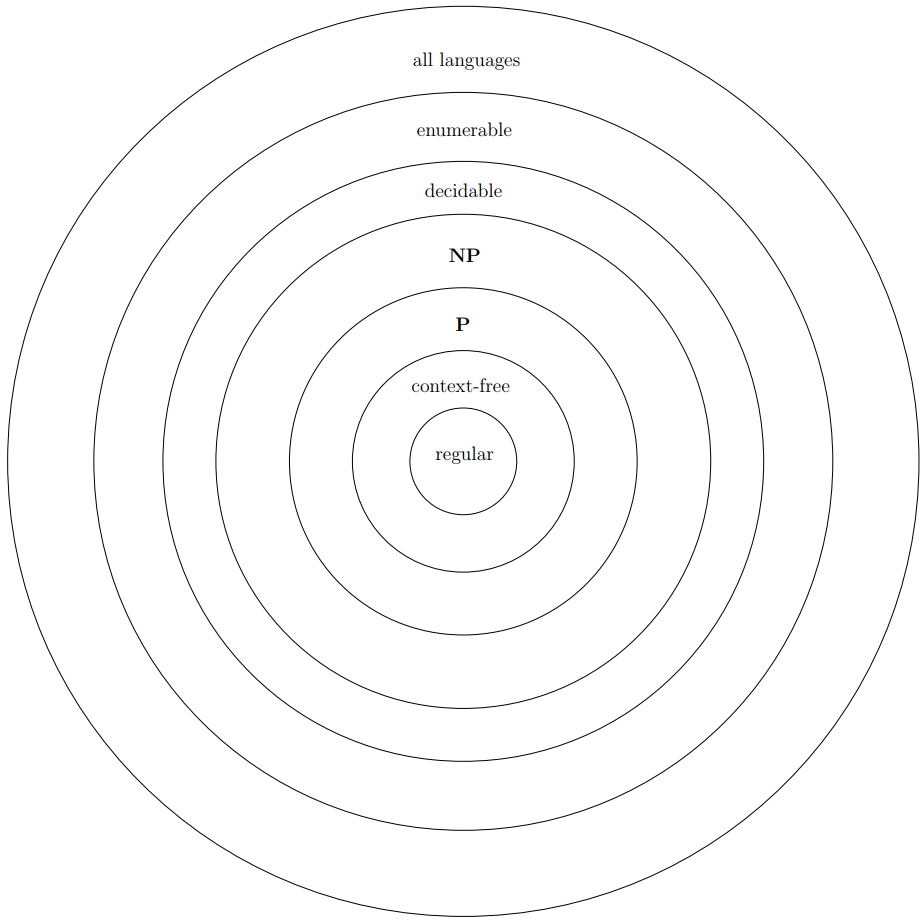
\includegraphics[width=0.7\textwidth]{../img/11-hierarchy.png}
        \blfootnote{Image from Maheshwari and Smid's \textit{Theory of Computation}, 2017}
    \end{center}
\end{frame}

\begin{frame}{El caso $a^nb^n$}{Lenguajes libres de contexto}
    \begin{block}{Tesis}
        Sean $L = \{a^nb^n, n \in \mathbb{N}\}$ y $LR$ el conjunto de los lenguajes regulares. Entonces, $L \not \in LR$.
    \end{block} \pause

    \bigskip

    Como un autómata debe tener un número \textit{finito} de estados, no hay manera de hacer que recuerde cuántas $a$s van para saber cuántas $b$s deberíamos tener.
\end{frame}

\section{Diferencias entre RGs y CFGs}

\begin{frame}{RGs y CFGs}{Diferencias entre RGs y CFGs}
    Las \alert{reglas} en una \textbf{RG} son del modo $A \to b\alert<4->{C}$ o $A \to b$. \pause

    \bigskip

    En una \textbf{Gramática Libre de Contexto} (GLC o CFG por sus siglas en inglés) las reglas son del modo $A \to b\alert<4->{C}d$ o $A \to b$. \pause

    \bigskip

    Además, incluimos nuevas reglas: $A \to \varepsilon$ \pause
\end{frame}

\section{CFGs bien formadas}

\begin{frame}{Volvemos al caso $a^nb^n$}{CFGs bien formadas}

    \textbf{Palabras aceptadas}: $\varepsilon, \alert<3->{ab}, \alert<4->{a}\alert<3->{ab}\alert<4->{b}, \alert<5->a\alert<4->{a}\alert<3->{ab}\alert<4->{b}\alert<5->{b}, \dots$ \pause

    \bigskip

    \only<2>{%
        ¿Qué patrón podemos identificar en los ejemplos? \pause
    }

    \only<6->{%
        \textbf{Estructura}: Grupos anidados de una $a$ al inicio y una $b$ al final.
    }

    \bigskip

    \only<7>{%
        \textbf{CFG}:
        \begin{enumerate}
            \itemsep1.5ex
            \item $S \to aSb$
            \item $S \to \varepsilon$
        \end{enumerate}
    }
    
\end{frame}

\begin{frame}{Ejemplo: \textit{Matching Parenthesis}}{CFGs bien formadas}
        \textbf{Ejemplos:} $(), (()), ()(), (())(), \dots$ \pause
        
        \bigskip

        \textbf{Estructura:}
        \begin{itemize}
            \item Grupos concatenados de paréntesis anidados $(((\dots)))$ \pause
            \item Cada grupo de $(((\dots)))$ es similar a $\{a^n b^n\}$ \pause
            \item<7-> Concatenamos usando una regla de tipo $S \to SS$
        \end{itemize}

        \bigskip

        \only<6>{%
            ¿Cómo concatenamos dos grupos?
            
            \bigskip
        }


        \onslide<4->{%
        \textbf{Reglas}:
        \begin{enumerate}
            \item $S \to (S)$ \pause
            \item $S \to ()$ \pause
            \item<8-> $S \to SS$
        \end{enumerate}
        }
\end{frame}

\begin{frame}{Ejemplo: expresiones aritméticas}{CFGs bien formadas}

    Podemos formar expresiones aritméticas también, como $25+3*12$, donde la multiplicación debe tener precedencia sobre la suma: \pause

    \begin{enumerate}
        \item $E \to E + T$ \pause
        \item $E \to T$ \pause
        \item $T \to T * F$ \pause
        \item $T \to F$ \pause
        \item $F \to CF$ \pause
        \item $F \to C$ \pause
        \item $C \to 0|1|2|3|4|5|6|7|8|9$
    \end{enumerate}

    \pause

    ¿Cómo derivamos $25 + 3 * 12$? \pause ¿Y $5 * 2 + 26$?
    
\end{frame}

\begin{frame}{Ejemplo: palíndromos en $\{a,b\}$}{CFGs bien formadas}
    \textbf{Ejemplos}: $\varepsilon, a, aa, aaa, aba, abba, \dots$ \pause

    \bigskip

    \only<2>{%
        ¿Cómo hacemos si es par, e.g. $abba$? \bigskip
    }

    \onslide<3->{%
        \textbf{Caso Par}: parecido a $\{a^n b^n\}$ pero con lo mismo en cada lado: $S \to aSa$ y $S \to bSb$, y usando $S \to \varepsilon$ para salir del \textit{loop}. \bigskip
    }

    \only<4>{%
        ¿Cómo hacemos si es impar, e.g. $abbba$? \bigskip
    }

    \onslide<5->{%
        \textbf{Caso impar}: idéntico al caso par, sólo que el \textit{loop} se termina con un terminal no vacío: $S \to a, S\to b$. \bigskip
    }

    \onslide<6->{%
        \begin{enumerate}
            \item $S \to aSa$
            \item $S \to bSb$
            \item $S \to a$
            \item $S \to b$
            \item $S \to \varepsilon$
        \end{enumerate}
    }

\end{frame}

\section{Operaciones en CFGs}

\begin{frame}{Combinación de CFGs}{Operaciones en CFGs}
    ¿Cómo \alert{unimos} dos CFGs? \pause

    \bigskip

    \textbf{Ejemplo}: CFG para las palabras de forma $a^nb^m$ tal que $n \neq m$ \pause

    \bigskip

    \textbf{Solución}:

    $$\{a^n b^m, n \neq m\} = \{a^n b^m, n > m\} \cup \{a ^n b ^m, n < m\}$$ \pause

    Usamos un \textbf{símbolo inicial nuevo} para hacer dos nuevas reglas: $S_0 \to S_1$ y $S_0 \to S_2$, donde $S_1$ y $S_2$ son los símbolos iniciales de las CFGs 1 y 2, respectivamente. \pause

    \bigskip

    La \alert{concatenación} es similar. Agregamos una nueva regla: $S_0 \to S_1S_2$.
\end{frame}

\begin{frame}{Ejemplo de ambigüedad: $\#a = \#b$}{Ambigüedad y Refinamiento de CFGs}
    \textbf{Estructura}: grupos de $a \dots b$ o $b \dots a$. \pause

    \bigskip

    \textbf{Reglas}:
    \begin{enumerate}
        \item $S \to aSb$
        \item $S \to bSa$
        \item $S \to SS$
        \item $S \to \varepsilon$
    \end{enumerate} \pause

    \bigskip

    Probar \textbf{derivaciones} usando \textit{DFS} para $abab = \langle 3, 1, 4, 1, 4  \rangle$ y $ abab = \langle 1, 2, 4 \rangle$.
\end{frame}

\begin{frame}{Eliminación de reglas}{Ambigüedad y Refinamiento de CFGs}
    Es posible reemplazar reglas en una CFG sin alterar el conjunto de palabras que se pueden formar con ellas. \pause

    \bigskip

    Por ejemplo, aquellas que generen producciones vacías: $A \to \varepsilon$ \pause

    \bigskip

    Producciones `inútiles' para reducir el tamaño de las derivaciones: $A \to B$ y $B \to a$.
\end{frame}

\begin{frame}{Eliminación de reglas}{Ambigüedad y Refinamiento de CFGs}
    Existen algunos problemas con las reglas vacías: \pause

    \bigskip

    Son \textbf{ineficientes}, pues crean un símbolo para después destruirlo. \pause

    \bigskip

    Las reglas vacías pueden \textbf{crecer o decrecer} las derivaciones, e.g. derivaciones de $ab$ \pause

    \bigskip

    $$S \to SS \to SSS \to SS \to SSS \to SS \to S \to aSb \to ab$$
\end{frame}

\begin{frame}{Eliminación de reglas vacías}{Ambigüedad y Refinamiento de CFGs}
    Para eliminar reglas de producciones vacías $A \to \varepsilon$, se reemplaza el lado derecho de cada ocurrencia de una regla: \pause

    \bigskip

    \begin{columns}
        \begin{column}{0.5\textwidth}
            \begin{enumerate}
                \item $S \to aSb$
                \item $S \to \varepsilon$
            \end{enumerate} \pause
        \end{column}
        \begin{column}{0.5\textwidth}
            \onslide<5->{%
                $$aabb = \langle 1, 1, 2 \rangle$$
            }
        \end{column}
    \end{columns}

    \bigskip

    donde podemos reemplazar cada $S$ por $\varepsilon$, para generar una nueva regla: \pause

    \bigskip

    \begin{columns}
        \begin{column}{0.5\textwidth}
            \begin{enumerate}
                \item $S \to aSb$
                \item $S \to ab$
            \end{enumerate} \pause
        \end{column}
        \begin{column}{0.5\textwidth}
            \onslide<6->{%
               $$aabb = \langle 1, 2 \rangle$$
            }
        \end{column}
    \end{columns}

    \bigskip

    \onslide<7->{%
        ¿Qué pasa si el lenguaje $L(G)$ sí contiene a la palabra vacía $\varepsilon$?
    }



\end{frame}

\begin{frame}{Eliminación de reglas `inútiles'}{Ambigüedad y Refinamiento de CFGs}

    Para eliminar las reglas `inútiles' (o pasos intermedios) en una CFG hay que ir \textbf{conectando} los extremos: \pause

    \bigskip

    \begin{enumerate}
        \item $S \to aSb$
        \item $S \to ab$
        \item \alert<3->{$S \to V$}
        \item \alert<3->{$V \to a$}
    \end{enumerate} \pause

    \bigskip

    \onslide<4->{%
        En lugar de tener dos reglas $S \to V$ y $V \to a$ podemos tener directamente una sola, $S \to a$:

        \bigskip
    }

    \onslide<5->{%
        \begin{enumerate}
            \item $S \to aSb$
            \item $S \to ab$
            \item \alert{$S \to a$}
        \end{enumerate}

        \bigskip
    }

    \onslide<6->{%
        ¿Qué pasa si hay ciclos en plan $S \to T$ y $T \to S$?
    }
    
\end{frame}

% \section*{Referencias}
% \begin{frame}[t]{Referencias}
% \nocite{bibID01}
% \nocite{bibID02}

% \bibliographystyle{IEEE}
% \bibliography{biblio}
% \end{frame}

\end{document}